 \section{Description and Analysis of the Domain}

The days of building websites that serve as static, digital pamphlet are long gone. Today, any information providing entities, including governments, are expected to provide constant, dynamic, customized, and shareable content. Without a tool that allows government website administrators to manage their own content, site updates can only be accomplished by a website developer with the tools and knowledge to write source code. To accomplish updates through such a vendor service model, governments must contract with a development company, submit requests, and wait days or even weeks for new site content and functionality to be online.

\subsection{The purpose and objectives of the project}
What can a website do for you, and for the government? First of all a website is a communication tool, it provides to users and government based in remote locations with a way to exchange and share information over the network.

Being more specifically, from the point of view of government a website can fulfill one or more functions. A website can be a publishing tool, such as a magazine, newspaper, radio, television by publishing about government various activities. Also a government website can be a marketing tool, promoting their services, activities or it may be used for building and enhancing the image of public institutions. For example, increasing the trust of the public for a new regulatory authority or promoting commercial services such as documentation services, activities of statistical office or sites that promote public libraries. Additionally governmental website can be a transactional tool, which allow the users and governmental institution to exchange all the information required to support a transaction. For example paying taxes, requesting licences or managing contracts. Also it can be a work tool, allowing a public agency to exchange information with its employees and thus facilitate professional activity. As an example websites with restricted access that allows police authorities to access the vehicle registration databases managed by transport authorities. Another example would be a site designed to make medical knowledge resources available to doctors.

Government institutions are interested in one or more of the possible use cases illustrated above and if planned and realised appropriately than a website can be a relatively inexpensive and efficient solution if compared with other methods of communication.

\subsection{Analysis of this field}
Like other media applications, a website is only one of variety of communication methods likely available to governmental organisations, which has its advantages and disadvantages.

Before investing in a website agencies first evaluate if communicating through a website is an appropriate and viable way to address their communication needs. Here are some examples of the advantages and disadvantages of using a website for this purpose.

Let’s begin with the most loveable benefit by our government, it is cheaper. A website can be a very cost effective way to exchange information, for both sides of monitor, for website’s owner and the end user. For instance, from the point of view of the government agency or institution a website can reduce the number of employees the agency or institution has to deal with, by providing answers to the most common queries or questions, also known as FAQs (Frequently Asked Questions), it normally receives, and so reduce the amount of employees effort and cost needed to answer them. Generally speaking a website makes it possible to publish extensive information on regulations, procedures and other aspects of an institute's work, which would otherwise need to be announced through direct human intervention, this means a governmental institute or agency can dedicate less staff time to dissemination activities, allowing either for a reduction in staff numbers, or for their employment elsewhere in the agency. Websites also represent a cheaper alternative to the production and dissemination of printed materials, like brochure, letters and so on. Also, it should always be considered that building and maintaining a website also has its costs, see disadvantages below, so agencies planning to use a website to try to cut staff costs should always make sure that the savings obtained to offset the cost in terms of staff and money necessary to build and maintain a web application. A website can also represent a cheaper communication alternative from the users point of view, especially if they are located in remote regions or abroad, as a phone call to an internet provider is often cheaper than a long-distance call, or a physical talk with the agency.

We all know the phrase “Time is money” and here step in another benefit which is quicker. Web publishing is immediate, and this enables agencies to introduce changes to their public easily and relatively quicker than with traditional and more costly methods depending on print. The immediacy of web publishing also allows the fast release of news and other information items to the public, which an agency may find advantageous, respond to promptings from the media, or act in moments of crisis. In addition to this, if maintained properly a website provides information 24 hours a day, 7 days a week, and can be available for the parts of the population either that find it hard to visit the agency in person, especially people with disabilities or those who cannot contact it during working hours. This can extend to providing the possibility to conduct transactions, for example requesting a licence, outside working hours and/or without visiting government offices, which can be useful in our country where travel is slow, costly or generally not easy. Conducting transactions online is also generally faster, as data can be recorded and transferred very quickly, as opposed to what happens with other, more traditional ways of handling bureaucratic procedures, such as paper-based forms, manual input by officials and so on.

 Websites can provide better ways to manage information compared to traditional means. Hypertext enables you to provide access to complex sets of information in relatively easy and user-friendly ways and combined with databases, it can also provide users with ways to interact directly with the data, for example to consult it, update it and/or send it to other destinations. In other words, a website can enable users to initiate and/or complete service transactions without recourse to human intervention. The absence of a gate keeping role on the part of humans not only saves time and money, but it is also likely to help reduce and prevent phenomena such as corruption, blackmail and bribery, a problem experienced by many governments, especially in our. By potentially cutting out "middlemen", websites represent a relatively transparent way of administering services and information, in comparison to traditional means. Having a website also provides governmental bodies with an opportunity to systematically collect information about their clients and users, this includes running surveys, asking users to share their personal data in order to register for specific services and therefore easily create and maintain a database of users of these services, and generally monitoring the behaviour of visitors to the site, for example through statistical analysis, which can be used to establish what information users are most interested in.

Websites provides a new, additional point of contact for the growing part of the population that uses the web. It is estimated that currently just over 47\% of the global population has access to the internet, an increase from just one year ago, when the same agency estimated that just over 43 percent of the global population were Internet users. That said, it should be considered that the percentage of internet users in developing countries is very often significantly lower than in developed countries, though it will increase slowly, in the next years. This means that agencies with international audiences such as donors, international institutions, and governments of other countries may be in a better position to exploit the potential of communicating on the web than those who deal directly with the local population. Implementing the use of email and/or online forms through a website also offers a fast and efficient alternative communication method for those who prefer indirect contact to communicating in person or on the phone for time or personal reasons. Basically, a website can generally introduce new ways of doing things , or new services altogether like paying your tax by credit card, which may have been too expensive via traditional channels because of the expenses connected to having card-reading machines. Finally, a website also represents an innovative tool for hiring new employees, providing agencies with a way to announce vacancies to a wide audience relatively cheaply, and therefore enlarge the potential base of recruitment, with the added bonus that those who apply via a website are likely to be in possession of some computing and web skills that could be put to good use in the organisation.

Now let’s look on the other side of the coin, disadvantages. Websites cost, building and maintaining governmental websites can require quite a lot of time and money. Apart from technical costs, there are also important human resource costs. Any existing or new staff working on the web must be trained both on the technical and communicational aspects of the new technologies they are to use. Agencies should therefore always factor in recruitment, training and other organisational costs when budgeting for a website, all of which can be particularly expensive in developing country contexts, where local capacities and expertise may not be sufficient, and trainers, consultants and technologies have to be called in from abroad.

Implementing the use of e-mail through an government website potentially leads to a new flow of enquiries from the public, through a different channel. Agencies should therefore ensure their organisational structure is capable of dealing with these communications in a timely and efficient way, especially considering that web users often expect quicker reaction and communication than those who communicate with traditional methods. It is hardly acceptable to adopt e-mail as an additional, fast method of communication and then leave emails unanswered for long periods of time. Again, this points to the costs mentioned in the previous point.

Web publishing usually represents an alternative and additional source of information to print publications, press releases and media broadcasts. It is essential that the entire information output by a governmental organisation is consistent and not contradictory, and adding an extra source like a website makes this even more complex, especially considering the immediacy of web publishing. This is particularly so when it comes to information with legal value such as laws or contracts, where discrepancies can cause serious issues.

Publishing information of legal value or granting access to information databases through a website can pose security dangers to governmental organisations, as malicious users, also known as hackers, can break into website systems through the internet and access, modify or delete information, up to and including making a website inaccessible, or deleting it completely. Defending your website from the attacks of hackers should be a priority, especially if it carries or gives access to legal or confidential information. All this leads to more costs in terms of software and expertise.

A website does not reach the entire population, but only the part of it that has access to the web. This is especially a problem in developing countries, where access to the internet is still often limited to a very small part of the population. Websites should therefore be considered only as alternative means of communication, and traditional methods of exchanging information should also be offered and maintained, at least until they become redundant as was recently the case with the telegraph.

How can government agencies reap the benefits of having a website and reduce the impact of the disadvantages outlined above? The answer lies in good planning. If web projects are planned and funded appropriately, they usually have higher chances of being a success.

\subsubsection{Planning}
You will agree that if a government agency decides to produce a new publication, or introduces a new system for paying tax, or an innovation in the way it works, it would be good practice to plan the operation as effectively and efficiently as possible, in order to reduce the risk of possible failures and the waste of public funds, if not worse, they generate.

The same can be said for websites. Building, developing and maintaining successful sites are all operations that require a good deal of investment in terms of time and money. Government agencies considering the adoption of a website as one of their communication tools should therefore make sure that the operation is planned appropriately, by giving particular attention to both the agency's and the user’s communication needs, and producing a sustainable and realistic project, in accordance with the resources at their disposal.

Planning your website properly will increase the chances of success, and save you a lot of money and resources, which can be limited in the context you work in. So, before you even start to design and implement a website, sit down and plan how to turn the project into reality with the resources you have at your disposal.

	A simple and effective approach to planning a website is to answer five basic questions:

	\begin{itemize}
		\item Why do you want to set up an Government website?
		\item Who is the website for?
		\item What information do you need to put on the website?
		\item Whom will you make responsible for it?
		\item How much can you spend on it?
	\end{itemize}

\paragraph{Why do you want to set up an Government website?}

Your website will be more likely to be successful if you set a series of clear objectives for it. These objectives can be improved if they are SMART: Specific, Measurable, Agree, Realistic and Timed.

Specific - setting goals as specifically as possible will enable you to provide clear guidelines on the features and functions that need to be implemented on your website, and therefore economise in terms of time and resources. For instance, instead of defining your goal as "providing information to the public", it would help to say "provide X type of information, to Y type of public, in Z format and at XYZ conditions". Indetermination in your objectives may lead to the realisation of an unfocused, confusing and potentially unsustainable web application.

Measurable - the objectives you set should be measurable. If, say, one of your objectives is "to reduce the time it usually takes to obtain a licence by half", for example by allowing the transfer of documents in electronic format through the site, rather than relying on traditional mail, you should make sure that the organisation you work for already has reliable methods in place to measure this reduction. In this case it would mean that you need to firstly, establish the average time taken to obtain a licence with traditional methods, and secondly record the time when the request is filed through your site, and the time of release of the licence, and compare this to the time taken with traditional methods: some of this requires the implementation of specific technical features in your website, and it is essential to establish this from the start.

Agreed - it is important that the objectives you set are agreed with the key stakeholders in your organisation, and particularly with management; this will provide you with common and formally accepted criteria to review the progress of the project in the future, and with the clarification of the different lines of accountability by the people involved in the project. If you obtain the sponsorship of key people in your organisation, you will also be in a better position to solicit resources for the project's realisation. Best practice would be also to include representatives of user groups in your discussions and consult them on their expectations from the website you intend to set up.

Realistic - agencies should make sure that they evaluate the skills and resources they have at their disposal, and plan accordingly; setting unachievable goals for an e-government website represents a waste of time and public resources. As an example, rather than aiming to handle all applications online, it may be better to aim to handle "at least 90\%" of applications this way.

Timed - it is valuable to set deadlines for the achievement of objectives, as it helps to measure the achievement of your objectives: "handle 90\% of enquiries online by 2018". Deadlines can be reviewed if priorities change or unforeseen difficulties arise, including technical problems, which can be quite common with websites. It is therefore important to also build some flexibility into their definition.

By consulting with the relevant people in your organisation, it is likely that you will come up with more than a single objective for your website. In this case, it can help to prioritise objectives.

Assigning different priorities to your goals will help you make important decisions that affect the design and implementation of your website. This will help especially if resources are poor: if you don't possess the necessary resources to achieve all goals, you can use what is at your disposal to obtain at least the most important ones.

For example, the prioritised goals for a public agency's website could be:

\begin{itemize}
	\item to publish a specific set of information in order to reduce the number of queries from the public,
	\item to enhance the profile of the institution in order to attract donors to collaborate with it, and
	\item to enable users to carry out online transactions with the authority.
\end{itemize}

If you only possess very limited resources, you may consider dropping the third goal or deferring it to a later stage of the life of the website, especially because it is likely to put heavy technical requirements on the project . If instead you had assigned top priority to online transactions, you would need to use most of your resources towards that goal, which may risk your chances of achieving the other ones.

The bottom line is that it is usually better to achieve a limited number of goals efficiently than to pursue a larger number of goals and only achieve them partially.

\paragraph{Who is the website for?}

After establishing the primary objectives for your website, you should focus on who the audience for your website is likely to be.

In fact, this is the factor that will have the biggest influence on the way you structure and design your site: you should always bear in mind that a website is primarily a communication tool, and that as such, it should be as easy and straightforward as possible to use for your intended audience. In other words, the way you organise and structure contents, the navigation system you implement, and the layout of the site should be as user-friendly as possible.
In real-life situations, and especially if you set multiple objectives for your website, it is likely that you will be looking at catering for a variety of users . In this case, it would help to prioritise users in different categories, as this will provide you with clear criteria for taking decisions in case you cannot satisfy the needs of all users with the resources you have at your disposal.

There are two main aspects it would help to focus on when you analyse who the users of the website could or should be: the type of activity they would be likely to be undertaking when visiting your website, and the user’s technical profile.

The activity users intend to undertake, or the informational needs they intend to satisfy when they visit your government website, will influence the way they use the website itself, and you should be prepared to take this into account when planning the site. In the case of government websites, main user profiles can be roughly divided into two categories:

\begin{itemize}
	\item Seekers of information: these users are looking for a specific piece of information, and they will browse the site until they succeed or fail, as such, they usually benefit from the implementation of site search features, indexes, sitemaps, and a hierarchical, category-based navigation system, which all help them to find the information they want more quickly. In order to cater for cases in which the information required cannot be found on the site, it would also help to supply e-mail contacts or indicate other communication channels through which enquiries can be made.
	\item Users in need of online services: these users are looking to undertake an online transaction through a website for example requesting a permit, or paying tax. They need to be pointed directly to this service, as carrying out the transaction itself is likely to require consulting a variety of web pages and completing different steps. Implementing direct links or buttons to services from the homepage, or from every page on the site, would reduce the time it takes for the transaction to be completed. Clear instructions and explanations for every step in the transaction are also very beneficial, and can foster the user’s trust of the application, and of the institution at large.
\end{itemize}

Technical skills, this includes both the technical setup your users are likely to be using when they access your website, and their skills and proficiency in using IT and alphabet-based communication tools.

Users in developing countries often have limited access to recent technologies, and access the web through relatively slow connections: it is therefore important that you design your website to be accessible also in these conditions. This means you should, for instance, avoid adopting very complex graphical designs and avoid relying on very large files to convey information.

The typical users of government websites may also be people with varying IT and general knowledge: this is especially the case if the site is designed to cater for a very wide section of the population. You should therefore make sure that the site is usable and comprehensible by most, if not all, users, including those whose skills and knowledge are limited. This means first of all using common language and clear, extensive instructions. But it also means that you may have to provide alternative routes for users, for example instructions for disabled people, or information in the different languages in use in your audience. If, instead, your typical users are specialists in a specific discipline, and your website is designed to cater for their needs, for example a website providing access to a medical knowledge resource database for doctors and hospital staff, you should make sure the terminology used in the site is specialised enough to be meaningful to them.

Failing to understand these requirements from the outset may lead to the need for an expensive and time-consuming review of the project later on, or to its ultimate failure.

\paragraph{What information do you need to put on the website?}

An government website is primarily a communication tool designed to facilitate the exchange of information between the public agency and citizens, or other parts of a society. The aim of this exchange of information is usually to support decisions, for example helping a citizen or an organisation to decide whether to apply for a public grant, or convincing a donor that they should fund a government project, or to facilitate a transaction, for example enabling a citizen to request a permit or licence. In short, government websites are there to support actions on the part of their users, by supplying all the information needed to take decisions, or finalise transactions.

You should therefore ask yourself what will the typical user be trying to do when visiting my website? What actions is she or he likely to want to undertake, to which the website could be of support?

This will help you establishing the type of information you should supply through your site. By running through what could be the typical decision-making processes of your users, you will be able to identify the information they require in order to make their decisions, and evaluate whether this can be supplied through your website.

For example, if one of the goals of your website is to help citizens decide whether to apply for a grant, you would probably need to provide:

\begin{itemize}
	\item a navigational system designed to direct users from the first page they consult to a page about the grant that would best fit their needs;
	\item 	general information about the aims and scope of the grant;
	\item information on the criteria of eligibility for the grant, both in terms of the applicant and the project to be funded;
	\item information on how to proceed with the request, and on the practical aspects of the application, of the awarding and of the transfer of funds, including deadlines and other time-sensitive information;
	\item the possibility to apply online, if this is possible;
	\item if relevant, information on alternative funding possibilities if the criteria for eligibility are not met, or the grant does not fit the needs of the applicant.
\end{itemize}

In the very likely case that you have set up a number of different, prioritised goals for your site, and have identified a number of prioritised groups of users, you will also have to assign priorities to the types of information you will need to supply through the site.

Reflecting on what information you should provide through your website is particularly important if you consider that sourcing, editing and managing contents is perhaps the most time-consuming and human resource-intensive aspect of the realisation of a web project: while design and technical implementation normally require the input of a relatively limited number of people, the production of relevant, up to date contents usually depends on the involvement of staff from different offices and departments in your institution, and needs to be planned efficiently, and fit into people's workloads. It is therefore essential that you focus on what the key requirements are in terms of contents for your site, and this is where prioritising types of information, and the formats in which they are made available, will be useful.

It should also be noted that in some cases you may want to provide particular pieces of information which may appear as being of secondary importance if compared to the core goals of the site, but which may help you attracting a larger number of users, which you can then try and direct towards the core functionalities of the site, for example in order to attract young people to a site that contains information about birth control or HIV prevention, it may help to also publish information that is relevant to other aspects of their life, such as entertainment or sport, which may not be entirely relevant to the ultimate objective of the site, but which could exercise an important "pulling" power for young users.

Whatever you choose to publish on your site, you should make sure that you set some priorities for the different types of contents, and that you actually are in possession of the information needed, or of efficient ways to obtain it from your organisation. And you should always put yourself in the position to review contents and priorities in the future, if the perceived users needs change after carrying out an evaluation, or survey.

\paragraph{Whom will you make responsible for it?}

Although it may be designed to help you reduce administrative work in some areas, you should always consider that a website will create work for your agency.

Staff resources will be needed not only to produce and launch the site at the start of the project, but also to maintain and review it in the long term, and to respond to the extra flow of enquiries through different channels it may generate.

However you decide to allocate the necessary staff resources for developing and running a website, you should make sure you think in a long-term perspective : you will need to find staffing solutions that fit with the agency's priorities and budgets in the long run, to make the project viable and sustainable.

There are three main areas of activity in the development and maintenance of a website, for which you should assign responsibilities:

Design and Development: elaboration of the structure and graphical layout of the site, implementation of the navigation system, creation of sample pages, also called templates, and other technical aspects connected to the creation of the site. This is not necessarily a permanent function: most of this work will in fact be done only at the start of the project, during which the person responsible for the project will need to work in close collaboration with whoever you have made responsible for it, be it internal to the agency or hired externally. But you should consider that you may need to review the design or implement new features later on, once the website is up and running, so you should always make sure you have access to the skills and resources needed to carry out this work if necessary.

Website Administration: day-to-day running of the site, including reviewing and updating contents and making sure that links, forms and other features of the site keep working. This is an essential aspect of the delivery of a website, as it guarantees that the site is online, that it works properly and that it provides the information you want it to provide, in a timely and accurate fashion. The management and oversight of a website are long-term operations which usually require medium to advanced technical skills, and are best carried out in-house, for example using resources internal to the organisation, for better immediacy and accuracy.

Content Provision: this aspect of producing and maintaining a website is often underrated, but it's a very important part of the process. Content should be uploaded regularly and kept up to date: relevant members of staff in your organisation should therefore commit to providing content for the areas in which they operate and on which they have knowledge and expertise. Remember, too, that website contents need to be adapted for publishing: writing for the web follows different rules than, say, writing for a magazine or writing a report, and you should make sure that someone in the organisation is trained to handle different types of contents and make them fit for publishing on the web.

To cover all these functions you will need to allocate resources and identify the people who will carry out the work, both in the short and in the long term. In order to do so, you should ask yourself the following questions:

In-house or outsourced?

For every aspect of the production of a website, you should choose whether it is more convenient and efficient to address it by using internal resources that can be made available within your organisation, in-house or by hiring another public agency or a private company to do it outsourcing. This depends very much on how important the website is for your organisation. Outsourcing can be expensive, as private companies generally charge hefty amounts of money for web work. If the website becomes a constant and essential feature of the agency's work and requires a constant input of resources, you would probably be better off using internal resources. You may also decide that you want to outsource some of the work, and keep in-house the rest. A typical example: the first stages of the design and implementation of a website are often assigned to professional web designers outside the organisation. The maintenance of servers, which can be complex and rather expensive to run, is also very often outsourced, unless the organisation is very large or needs to control their servers directly, for security or legal reasons. Content management is instead often done in-house, as it requires knowledge and expertise that can be found more easily within the organisation than outside it.

In the case of in-house solutions, you should evaluate whether it is possible to assign tasks to existing staff, or if you need to employ new staff. This depends on the workload generated by the website: if this can be sustainably integrated into present workloads, then you may choose to work with existing staff. But it is likely that you will need extra resources to run a website properly, so you should also consider employing new staff. This doesn't necessarily mean employing a new person to work on the web, perhaps one or more current employees possess the necessary skills, or are willing to develop them, the bonus in this case is that they already know the organisation very well. They could therefore be the right person for the job, so you might want to give them new web-related positions, and recruit new staff to cover the one they are leaving vacant. Training and redeploying existing staff may also be an interesting solution for organisations undergoing reform and restructuring, as it may help in finding a new role for members of staff that may otherwise become redundant.

However you decide to allocate the necessary resources for developing and running a website, you should always make sure that you do so in a long term perspective. While a website can be quite expensive and resource intensive to set up at first, if you want it to be successful you will have to take into account a constant effort, both in terms of time and money. Regular reviews and updates of contents are essential, as is the general maintenance of the site. If you opt for in-house solutions, you can try to make sure that website related tasks are integrated into the job descriptions of the staff you employ, and that sufficient time and incentives are provided in order to carry them out. Don't leave this to improvisation: it's a recipe for disaster. If no one has the time to work on the site, this will become unusable and will detract from the overall image of the organisation. Like all other operations within your organisation, creating and running a website must be sustainable, if it is to be a success.

\paragraph{How much can you spend on it?}

Creating and maintaining a website costs money, and you should make sure you budget for these costs appropriately. Most of the expenses are human resource-related, but you should also budget for technical costs, and unforeseen circumstances, as technical problems, unexpected requirements, training due to staff turnover and so on.

Building the necessary skills to construct and maintain a website can be pretty expensive, especially if you choose to hire external companies to do part of the work.

Opting for in-house solutions may appear less expensive, but it may turn out to represent an important cost in the long term, especially if you choose to employ new staff. And even if you decide to only use existing staff, they will need to be trained to do the job, and will not be in the position to contribute to the rest of the organisation's work during training, so you should factor that in when you budget for the project.

Opting for outsourced solutions does not entirely eliminate internal costs, as staff internal to the organisation will have to set up tenders and manage relationships with the company or companies chosen to do the work. Liaising and collaborating with external companies in order to explain what your organisation needs, and managing this relationship, can also be rather demanding, especially in the initial phases of the project. Often the amount of time needed for planning and setting up the site is underestimated: make sure you don't make this mistake.

There are obviously some technical costs you have to take into account when it comes to producing and maintaining a website:

\begin{itemize}
	\item hardware costs (computers for internal staff, printers, scanners, connections etc.).
	\item software costs (web design software, content editing software, picture editing software): avoiding such costs by trying to use pirated software can be particularly inappropriate for a government organisation.
	\item hosting costs: unless you decide to implement your own servers, which has itself its own costs in terms of hardware, software and maintenance or a central public agency can provide hosting for you, you will have to pay for commercial web hosting services, pay a company to provide file storage and to connect the site to the internet.
	\item technical support costs (technical help in case of software or hardware failures, general maintenance).
	\item domain name registration costs: the address of a site must be registered with the relevant authorities. Depending on national arrangements, this may be free of charge for governmental organisations, if not, you will have to pay a company to register and handle the web address or domain name for you.
	\item promotion costs: the cost of publicising and promoting the website, especially when it is first launched. It is no good creating a website and letting no one know about it: you will need to spend money in order to make the public aware it exists.
\end{itemize}

Nowadays governmental institutions usually face important financial constraints, and have limited resources at their disposal. This is especially true in developing countries. It is therefore likely that you will not be able to command princely sums to create and develop your website, and that you will have to work with a tight budget.

When budgeting for the project, you should therefore try to establish a balance between, what you ideally want to do with your website and so, ideally, how much you would need to spend on it. How much you can justify as a basic and fundamental need, without which the basic features of the project cannot be implemented.

This balance depends on a variety of factors, such as the goals you set for the website, and the level of sponsorship and support you manage to obtain for the project inside and outside your organisation. This is also where setting priorities for your goals will prove most useful. If the budget only covers a part of the goals, you should concentrate on the most important ones, and drop other, secondary goals, or defer them to a later stage, when the business benefits of having a website can be proven and you are in a better position to solicit more resources. If the budget available does not even allow you to achieve the most basic and primary goals of your website, the project might have to wait, or you might consider modifying its goals, or catering for a more restricted category of users.

In order to make the case for specific budgets to be put aside for the realisation of a website, you will probably need to demonstrate how this investment can be beneficial for the agency, and how it may lead to savings, or increase the agency's income by attracting donors, or combating tax evasion by providing easier ways to pay tax. When you do this, a full calculation would make sure you offset any benefits with the real expenses of creating and maintaining a website, especially in the long term.

\subsection{Project Analysis}
Thanks to advance in content management systems, governments no longer need to depend on IT companies to support with updates. Using a content management system, government website administrators without any knowledge in code editing, they can successfully update content, events,  images, documents, videos, and other dynamic media by themselves.

Aside from ease of use, timeliness and data storage, a CMS offers governments the next benefits.

“True genius lies in simplicity”, in a society where constant access to the latest information is requested and expected, governments must be able to easily and immediately to provide information to citizens, especially when it comes to emergencies, weather, traffic, election results, and other time sensitive information. Having a CMS that is easy to use and easy to update can save government’s time and money. 

In an intuitive content management system, the content and design lives in isolated functionalities. When is set with specific permissions, each feature would allow website administrators to work with content without fear of accidentally changing the overall website design.

Governments require to comply with government resolution number 188 of the 3 april 2012. It's vital for websites to provide the capabilities needed to ensure content is easily accessible by everyone. Not meeting website guidelines for accessibility could raise legal issues between citizens and government authorities.

On the rise of cyberattacks, it's becoming more important to protect government websites from data breaches and risk exposure. Without a secure CMS municipalities are exposed to any loss and theft of information taken from the website. Using a CMS with multiple levels of security to reduce and cover a cyberattack can save government institutions from the loss of money, time and reputation. 

Partnering with a government website design company, such as Center of Special Telecommunications, that offers access to a CMS and hosting will help to avoid much of the technical work needed for housing your site. The most valuable partners will be able to support your hosting needs with advanced data center technology supported by redundant networks, firewalls, and network providers, to help keep your information online 24/7.

The most important functions of your government website is its ability to equip citizens with online services that can save them time from coming into the office. Services such as bill payment, employment submissions, program registrations and facility reservations can easily be done online from the convenience of their home or on any mobile device. An engaging CMS solution that provides online services prevents the need for multiple third-party software integrations.

A CMS functions as a repository for every type of content made available to citizens. Partnering with multiple vendors to plug-in tools for document access, video players, photo galleries, calendars, etc. can lead to integration incompatibilities, and vendor management headaches. Working with one CMS to handle all digital requirements allows your website administrator to self-manage all content types using one intuitive solution with one contact for support services.

There are several providers out there that specialize in developing websites. However, the needs of businesses and bloggers is far different than that of a city or county. Having a CMS and website provider specifically focused on local government’s needs can save you a lot of time, money and headaches in the end.

\subsubsection{Drupal}
Developing a website from zero is difficult job that requires a lot of time. Using a CMS simplifies your job as web developer. There are lots of content management systems that provides many features. Of course all of them have advantages and disadvantages. Few examples of CMS that you might heard about is Wordpress, Joomla and Drupal. Those are the most popular CMS at the moment, firstly because they are open source. This project is based on Drupal, naturally you might want to know why, the answer is simple:

''Simplicity is the ultimate sophistication.''
- Clare Boothe Luce

The biggest disadvantage of Drupal is hard to learn, but when you get used to work with Drupal, you will be able to do amazing things that cannot be implemented in other content management systems.

\begin{figure}[H]
\centering
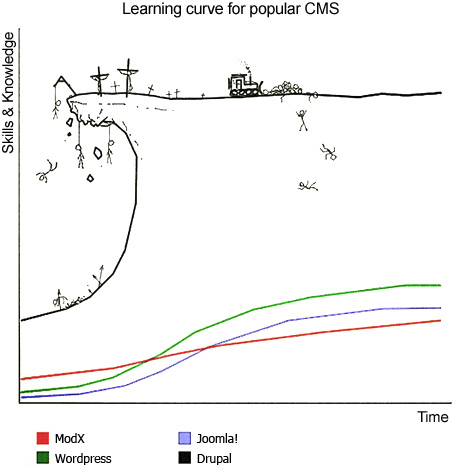
\includegraphics[width=14cm]{Chapter1/cms_learning_curve.jpg}
\caption{CMS learning curve}
\label{fig:cms_learning_curve}
\end{figure}

From content manager’s perspective it will be simple and intuitive to use features provided by developers. There are some standard requests from government and developing those requests takes time. The main goal of this project is to automate and simplify the process of creating new website for Moldavian Government.

\subsubsection{mGov}
Introducing the result of this project, mGov is a Drupal distribution developed specifically to meet Moldavian Government website guidelines. mGov uses Drupal 8, the latest and most advanced version of the Drupal CMS platform. Give your users a cutting edge digital experience with the power of open source. This latest version of Drupal gives you the option of custom website CMS functionality and integrates with third party tools when you need them. 

mGov meets all Moldavian Government website requirements, so when you install mGov you can be confident that your Moldavian Government CMS is equipped to grow with future developments in Drupal 8 and beyond.

Here are some of the mGov’s CMS platform specifications:

\begin{itemize}
	\item it is complete open source and follows Drupal security and coding standards;
	\item pre-packed installer with Drupal functional modeulws and front-end themes;
	\item completely extensible with any Drupal 8 modules or custom modules developed for specific features;
	\item it is designed to give you full control over installation and management;
\end{itemize}

\paragraph{Saves your time and effort}

mGov saves your time and effort by allowing to move quickly to create a seamless website experience with mGov’s ready to go features. From downloading to hosting, from transferring content to customising and organising your Government website, you’ll quickly speed ahead.

aGov can be installed on the hosting platform of your choice in under 10 minutes, and provides a fully featured Drupal 8 website out of the box, while meeting all Moldavian Government website standards. The advanced content management features will help you to collaboratively keep track of documents, page changes and other day to day activity with ease.

Focus your time and effort on creating engaging content and customised features. Because your Government Drupal site comes fully loaded with a core set of user interface elements, functionality and features - these can be reused as the basis for any new Moldavian Government website.

For small Government websites, the majority of requirements have been met in the out of the box version of mGov. Once it's installed, you're ready to go. For larger, more complex websites, you will have all the tools you need for customising and enhancing the features on your website.

\paragraph{Improved Performance}

Improve the performance of your website as you go. Get detailed insights into what works and what doesn’t for your users, then easily update and change anything and everything you need to.

To analyse how your website performs, simply synchronise with Google Analytics out of the box, or easily extend it with modules for most major analytics systems.

It makes sense to have full control of your website, and mGov is a Government website CMS that is entirely yours with no strings attached. You can configure all content without compromise, including terms and conditions, accessibility, contact details and copyright notices. With just a few clicks, your navigation can be easily restructured and new sections added.

\subsection{Comparing with other systems}
From perspectives of features this project is unique, yes there are similarities with other projects that are developed for other governments. Drupal is pretty widely used for building government websites.
